\documentclass[conference,a4paper,flushend]{cs-techrep}
\pdfoutput=1 % pdflatex hint for arxiv.org (within first 5 lines)

% Class cs-techrep.cls loads biblatex / biber with predefined options
\addbibresource{embedded.bib}       % its content is declared below, embedded within this tex-file
\addbibresource{webdev_commons.bib} % includes REST, React, Angular, Vue, Svelte, Docker, AWS-*, Socket.IO, and many more!
\addbibresource{cpn_all_all.bib}    % includes all previous CyberLytics@OTH-AW technical reports
\usepackage{graphicx} % Für das Einbinden von Bildern
\usepackage{titlesec} % Für das Anpassen von Überschriftenabständen

% Anpassung der Abstände zwischen den Überschriften
\titlespacing*{\section}{0pt}{*1}{*0.5}
\titlespacing*{\subsection}{0pt}{*0.5}{*0.25}

% ======================================================================
% EDIT THESE:

\cstechrepAuthorListTex{Juliana Kühn, Nikolett Rácz, Raffael Friedl, Maximilian Lippmann,\\ Christoph P.\ Neumann\,\orcidlink{0000-0002-5936-631X}}
\cstechrepAuthorListBib{Juliana Kühn and Nikolett Rácz and Raffael Friedl and Maximilian Lippmann and Christoph P. Neumann}

% Capitalization: https://capitalizemytitle.com/style/Chicago/
\cstechrepTitleTex{MunchMunch: Eine MERN-basierte kulinarische Web-Anwendung für verbessertes User Engagement beim Entdecken neuer Gerichte und Rezepte}
 % IF you need manual linebreaks in the titel, then clone the title without linebreaks for BibTeX:
\cstechrepTitleBib{{\cstechrepTitleTex}}

\cstechrepDepartment{CyberLytics\-/Lab at the Department of Electrical Engineering, Media, and Computer Science}
%\cstechrepDepartment{CyberLytics\-/Lab an der Fakultät Elektrotechnik, Medien und Informatik} % DE
\cstechrepInstitution{Ostbayerische Technische Hochschule Amberg\-/Weiden}
\cstechrepAddress{Amberg, Germany}
%\cstechrepAddress{Amberg, Deutschland} % DE
\cstechrepSeries{Technical Report}
%\cstechrepSeries{Technische Berichte} % DE
\cstechrepYear{2024}
\cstechrepMonth{6}
\cstechrepNumber{CL-\cstechrepYear{}-42}
%\cstechrepLang{english}  % en-US
\cstechrepLang{ngerman} % DE

% Special remark on babel/csquotes terminology in regard with US-vs-UK:
% en-US  = [english]/[american]/[usenglish] (+ [canadian])
% en-UK  =           [british] /[ukenglish] (+ [australian]) <OXFORD>
% For cs-techrep (like ACM), the recommended english variant is en-US!

% DO NOT DELETE THIS:
\filecontentsForceExpansion|[] % force command expansion inside a filecontents* environment
\begin{filecontents*}[overwrite]{selfref.bib}
    @TECHREPORT{selfref,
        author = {|cstechrepAuthorListBib},
        title  = {\cstechrepTitleBib},
        institution = {\cstechrepInstitution, \cstechrepDepartment},
        series = {\cstechrepSeries},
        number = {\cstechrepNumber},
        year   = {|cstechrepYear},
        month  = {|cstechrepMonth},
        langid  = {|cstechrepLang},
    }
\end{filecontents*}

% ======================================================================
% EDIT THIS:

\begin{filecontents}[overwrite]{embedded.bib}
@online{ieee2015howto,
    author = {Michael Shell},
    title = {How to Use the {IEEEtran} \LaTeX\ Class},
    url = {http://mirrors.ctan.org/macros/latex/contrib/IEEEtran/IEEEtran_HOWTO.pdf},
    year = {2015}
}
@online{ieee2018formattingrules,
    author = {{IEEE}},
    title = {Conference Template and Formatting Specifications},
    url = {https://www.ieee.org/content/dam/ieee-org/ieee/web/org/conferences/Conference-template-A4.doc},
    year = {2018}
}
@online{iaria2014formattingrules,
    author = {{IARIA}},
    title = {Formatting Rules},
    url = {http://www.iaria.org/formatting.doc},
    year = {2014}
}
@online{iaria2009editorialrules,
    _author = {Cosmin Dini},
    author = {{IARIA}},
    title = {Editorial Rules},
    url = {https://www.iaria.org/editorialrules.html},
    year = {2009}
}
@online{languagetool,
    author = {{LanguageTooler GmbH}},
    title  = {{LangueTool}},
    url    = {https://languagetool.org/overleaf}
}
@online{overleaf,
    author = {{Digital Science UK Limited}},
    title  = {{Overleaf}},
    url    = {https://www.overleaf.com}
}
\end{filecontents}

\usepackage{fontawesome} % i.a., \faWarning{}
\usepackage{relsize}     % i.a., \textsmaller{...}
\usepackage{lipsum}      % for blindtext

% ======================================================================

% cf. https://ctan.org/pkg/acronym
% Usage:
% singular, within sentence       = \ac{gui}
% singular, beginning of sentence = \Ac{gui}
% plural, within sentence         = \acp{gui}
% plural, beginning of sentence   = \Acp{gui}
\begin{acronym}
    \acro{gui}[GUI]{Graphical User Interface}
    \acro{ide}[IDE]{Integrated Development Environment}
\end{acronym}

% https://www.silbentrennung24.de/
% https://www.hyphenation24.com/
\hyphenation{block-chain block-chains Ethe-re-um}

\begin{document}
\selectlanguage{\cstechrepLang}

\maketitle

\begin{abstract}
MunchMunch realisiert eine MERN-basierte Applikation zur Förderung der kulinarischen Bildung und Optimierung des Kocherlebnisses. Die Anwendung bietet Funktionen zur Entdeckung, Speicherung und Personalisierung von Gerichten. Nutzer können bevorzugte Speisen speichern und auf zugängliche Rezepte mit detaillierten Zutatenlisten und schrittweisen Anleitungen zugreifen, die den Kochprozess vereinfachen. Die Motivation hinter dieser Anwendung liegt in der zunehmenden Nachfrage nach digitalen Hilfsmitteln für das Kochen und die kulinarische Bildung. Die Architekturziele umfassen eine benutzerfreundliche und intuitive Oberfläche, sowie eine robuste und skalierbare Anwendungs-Infrastruktur. Die Lösungsstrategie basiert auf dem MERN-Stack (MongoDB, Express.js, React, Node.js), wobei das Frontend für die Anzeige und Interaktion zuständig ist und das Backend die Geschäftslogik verwaltet. Die Kommunikation zwischen Frontend und Backend erfolgt über eine RESTful API.
\end{abstract}

% A list of IEEE Computer Society appoved keywords can be obtained at
% http://www.computer.org/mc/keywords/keywords.htm
\begin{IEEEkeywords}
Web technologies; MERN; Web server; User interfaces; React; Node.js; Express.js; RESTful API.
\end{IEEEkeywords}

\section{Problemstellung}
Die MERN-basierte Anwendung „MunchMunch“ wird entwickelt, um die kulinarische Bildung zu fördern und das Kocherlebnis zu optimieren. Nutzer können maßgeschneiderte und geschmackvolle Gerichte entdecken, Lieblingsspeisen speichern und auf zugängliche Rezepte mit detaillierten Zutatenlisten und schrittweisen Anleitungen zugreifen.
Das MVP (Minimum Viable Product) umfasst folgende Punkte:
\begin{enumerate}
\item  Registrierung und Anmeldung von Nutzern
\item  Anzeige von Essensvorschlägen aus verschiedenen Kategorien
\item  Suche- und Filterfunktion für Rezepte
\item  Detaillierte Rezepte mit Zutatenlisten und Anleitungen
\item  Favoritenfunktion für Rezepte
\end{enumerate}
Sind alle diese Punkte erfüllt, ist der User in der Lage die Applikation zu nutzen. Nachdem diese abgeschlossen sind, kann die Anwendung erweitert werden. Geplante, aber noch nicht umgesetzte Erweiterungen, sind im Abschnitt „Fazit und Ausblick“ beschrieben.
Netflix\cite{Netflix} und EAT CLUB\cite{EATCLUB} dienen als Inspiration für die aktuelle Entwicklung. Der Quellcode von MunchMunch ist im Open-Source Format unter der MIT Lizenz veröffentlicht.
\subsection{Mission Statment}
Eine gesunde Ernährung ist essenziell für das menschliche Wohlbefinden. MunchMunch macht es sich zur Aufgabe, dem Nutzer einen möglichst einfachen Zugang zu gesunden Rezepten zur Verfügung zu stellen. Durch detaillierte Rezepte soll der User in der Lage sein, jedes Rezept zu kochen. Such- und Filterfunktionen ermöglichen es dem User, Rezepte nach jeders Geschmack zu finden. Als User möchte man außerdem in der Lage sein, seine Lieblingsrezepte zu speichern, um diese später schnell und einfach zur Hand zu haben.
\subsection{Stakeholder}
Es gibt verschiedene Stakeholder, für die MunchMunch interessant ist.  
\begin{enumerate}
\item \textbf{Singles}: Singles leben oft alleine und suchen nach einfachen, aber leckeren Rezepten, die für eine Person geeignet sind. Sie schätzen schnelle und unkomplizierte Kochanleitungen. MunchMunch kann in diesem Fall helfen, personalisierte Rezepte vorzuschlagen und einfache Schritt-für-Schritt-Anleitungen bereitzustellen.

\item \textbf{Hobbyköche:} Hobbyköche haben Spaß am Kochen und experimentieren gerne mit neuen Rezepten und Techniken. Sie suchen oft nach Inspiration und möchten ihre Fähigkeiten erweitern. Sie suchen nach vielfältigen Rezepten, detaillierten Anleitungen und Informationen zu fortgeschrittenen Kochtechniken.
MunchMunch stellt eine große Auswahl an Rezepten, welche die Möglichkeit bieten, in den eigenen Lieblingsgerichten gespeichert und geteilt zu werden.

\item \textbf{Feinschmecker:} Feinschmecker legen großen Wert auf hochwertige Zutaten und raffinierte Gerichte. Sie sind oft auf der Suche nach neuen Geschmackserlebnissen und Trends in der Kulinarik. Sie wollen hochwertige Rezepte, ausgefallene Zutaten und Informationen zu neuen kulinarischen Trends. MunchMunch bietet Zugang zu exklusiven und ausgefallenen Rezepten und Empfehlungen für hochwertige Zutaten 

\item \textbf{Professionelle Köche:} Professionelle Köche haben eine fundierte Ausbildung und arbeiten in der Gastronomie. Sie suchen nach Plattformen, um neue Rezepte zu entdecken. Sie können MunchMunch nutzten um einzigartige Rezepte kennenzulernen.

\item \textbf{Hausmänner und Hausfrauen:} Hausmänner und Hausfrauen kochen regelmäßig für ihre Familie und suchen nach ausgewogenen, gesunden und schmackhaften Rezepten, die für die ganze Familie geeignet sind und allen schmecken. MunchMunch kann dabei helfen die Lieblingsrezepte zu speichern und bietet eine große Auswahl an verschiedenen Rezepten.
\hfill \break
MunchMunch bietet somit für jeden dieser Stakeholder spezifische Vorteile, die das Kocherlebnis bereichern und an die individuellen Bedürfnisse und Vorlieben angepasst sind.

\end{enumerate}
\section{Vorgehensweise}
\subsection{Kontextabgrenzung}
Die kulinarische Plattform greift auf eine manuell gepflegte Datenbank mit Rezepten zu. Diese Rezepte sind in verschiedene Kategorien unterteilt, die im Dashboard übersichtlich dargestellt werden. Nutzer haben die Möglichkeit, ein Konto zu erstellen, Rezepte zu favorisieren und zu speichern. Alle Nutzerinformationen werden sicher in der Datenbank verwaltet.
\begin{figure}[h]
    \centering
    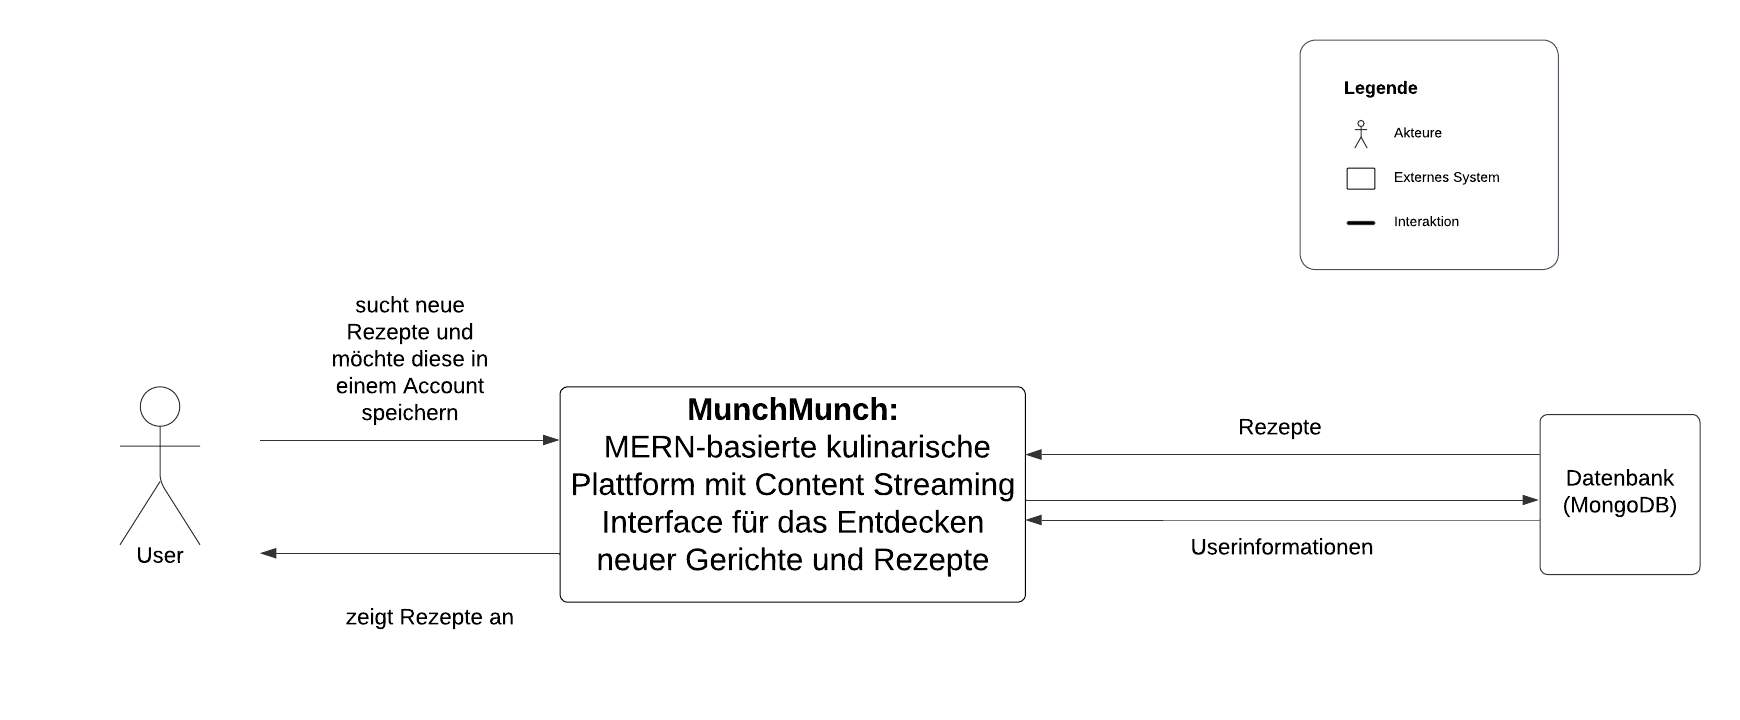
\includegraphics[width=1\linewidth]{Konzeptabgrenzung_Diagramm.png}
    \caption{Kontextabgrenzung des MunchMunch Gesamtsystems}
    \label{fig:enter-label}
\end{figure}

\subsection{Qualitätsziele}
\begin{tabular}{|p{3.5cm}|p{3.5cm}|}
\hline 
\textbf{Qualitätsziel} & \textbf{Erklärung} \\ % Kopfzeile der Tabelle
\hline % Horizontale Linie unter der Kopfzeile
Übersichtlichkeit & Klare, nicht mit Informationen überflutete Übersicht der Rezepte unterteilt in verschiedene Kategorien \\ % Erste Datenzeile
\hline % Horizontale Linie nach der ersten Datenzeile
Intuitive Bedienung & User weiß sofort wie Plattform zu bedienen ist \\ % Zweite Datenzeile
\hline % Horizontale Linie nach der ersten Datenzeile
Responsiveness  & Plattform soll auf jedem Endgerät bedienbar sein \\ % Zweite Datenzeile
\hline % Horizontale Linie nach der ersten Datenzeile
Sicherheit  & Authentifizierung erfolgt über einen Token und das Passwort wird gehasht \\ % Zweite Datenzeile
\hline % Horizontale Linie nach der ersten Datenzeile
Performance  & Daten und Bilder werden vom Backend an das Frontend übermittelt \\ % Zweite Datenzeile
\hline % Horizontale Linie nach der zweiten Datenzeile
\end{tabular}

\section{Randbedingungen}
Bevor die Entwicklung der Plattform beginnen konnte, mussten einige Randbedingungen festgelegt werden, damit die Plattform auf jedem Rechner eines Entwicklermitglieds läuft, und später für die breiteste Masse der Zielgruppe verfügbar sein kann.

\subsection{Technische Randbedingungen}
Wichtig war, dass die Anwendung möglichst viele Nutzer erreichen kann. Deshalb wurde als Plattform der Applikation eine Web-Anwendung gewählt, welche mittels Responsive Design auf Heimcomputern, Tablets und Smartphones gleichermaßen verfügbar sein soll.
Die genutzte Entwicklungsumgebung ist WebStorms von JetBrains und als Versionskontrolle wurde ein Repository auf GitHub angelegt. Dort wurden auch die Issues festgehalten und dem jeweiligen Entwickler zugewiesen. Für Icons wurde die Bibliothek Fontawesome verwendet.

\subsection{Organisatorische Randbedingungen}
Es wurde jeden Montag ein Weekly-Meeting vor der Feedback-Session abgehalten, in dem besprochen wurde, was seit dem letzten Meeting passiert ist und was für diese Woche zu tun ist. Dabei sollte jedes Teammitglied anwesend sein, sofern es nicht aus anderen Gründen verhindert war. Ein paar Aufgabenstellungen wurde gemeinsam im Team erledigt, da die Struktur dieses Projektes für jeden neu war und man so gemeinsam eine Lösung finden konnte.

\subsection{Codier-Richtlinien}
Es wurden folgende Richtlinien im Team festgelegt, damit am Ende der Programm-Code ein einheitliches Bild abgibt:

\begin{itemize}
    \item Neue Branches müssen folgende Nennung haben: „iss(Issue-Nummer)\_dev\_(Kürzel des Teammitglieds)”
    \item Programm-Code und Kommentare werden auf Englisch geschrieben.
    \item Methoden, Variablen und Ordnernamen werden in „camelCase” geschrieben.
    \item Typen, Klassen und React-Komponenten werden hingegen in „PascalCase” notiert.
\end{itemize}

\section{Lösungsstrategien}
Für den Technologie-Stack wurde der MERN-Stack gewählt. Dieser umfasst React.js\cite{React.js} für das Frontend, Node.js\cite{Node.js} mit Express.js\cite{Express} für das Backend sowie MongoDB\cite{MongoDB} als Datenbank. Zudem wird sowohl im Frontend als auch im Backend TypeScript\cite{TypeScript} verwendet, um die Vorteile statischer Typisierung und verbesserter Code-Qualität zu nutzen. Vite\cite{Vite} wird als Build-Tool und Entwicklungsserver verwendet, um schnelle Entwicklungszyklen und eine optimale Performance zu gewährleisten. Die Anwendung wird mittels Docker\cite{Docker} containerisiert und als Pipeline eingesetzt, um das Projekt automatisch von GitHub auf eine Amazon EC2-Instanz zu pushen und auf die Liveadresse zu deployen. Mit React.js werden die interaktiven Benutzeroberflächen entwickelt, während Node.js und Express.js robuste APIs ermöglichen. Die Datenbank MongoDB bietet Flexibilität und Skalierbarkeit für die Datenverwaltung. TypeScript trägt dazu bei, die Wartbarkeit und Lesbarkeit des Codes zu verbessern und frühzeitig Fehler zu erkennen. Für die Gestaltung der Benutzeroberfläche wurden kontinuierlich mit dem UI/UX Design Tool Figma Prototypen erstellt, damit alle Entwickler für den Aufbau des Systems eine einheitliche Grundlage haben und die gemeinsame Vision zu verbildlichen.

\begin{figure}[h]
    \centering
    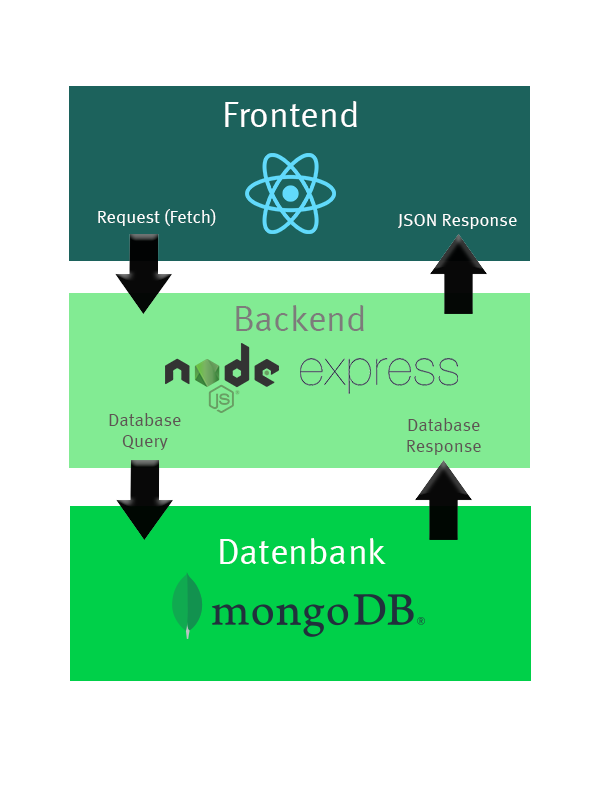
\includegraphics[width=1\linewidth]{systemueberblick.png}
    \caption{Systemüberblick visuell dargestellt}
    \label{fig:enter-label}
\end{figure}

\subsection{Datenbankarchitektur}
Für die Speicherung von Daten wurde eine NoSQL, dokumentbasierte, Datenbank MongoDB verwendet. Als Hosting-Provider wurde der Clouddienst MongoDB Atlas verwendet. In der Datenbank werden die Speisen in der Collection Meals mit dem dazugehörigen Rezept in Recipe gespeichert. Die Entscheidung wurde getroffen, um später die Gerichte mit weiteren Rezepte erweitern zu können. Außerdem kann der Benutzer sich registrieren. Mit dem angelegten Konto hat der Benutzer die Möglichkeit, die Gerichte und ihre dazugehörigen Rezepte zu speichern.
\begin{figure}[h]
    \centering
    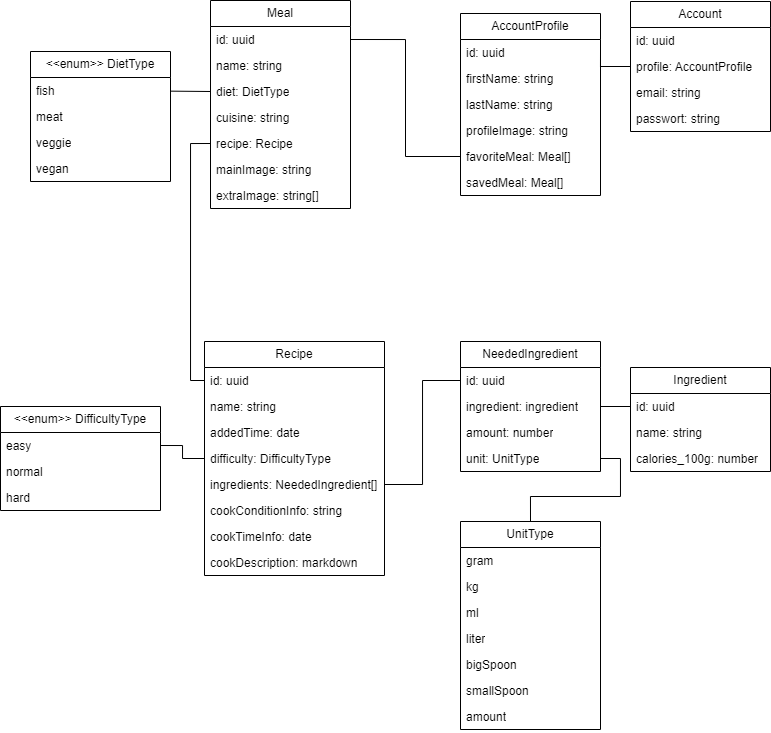
\includegraphics[width=1\linewidth]{datamodell.png}
    \caption{Datenmodell visuell dargestellt}
    \label{fig:enter-label}
\end{figure}

\subsection{Backend-Architektur}
Das Backend wurde als Node.js-Server implementiert, wobei Express.js für das Routing genutzt wird.
TypeScript dient als primäre Programmiersprache. Es setzt sich aus folgenden
Komponenten zusammen:
\begin{enumerate}
\item \textbf{Serverstart} : Der Serverstart  finden in
src/index.ts statt.
\item \textbf{Konfiguration}: Dateien server/src/config/config.ts, server/src/config/.env, server/src/config/.env.development, 
und server/src/config/.env.production enthalten die Konfiguration der Applikation. Sie beinhaltet die
Integration von Middlewares, Routeneinbindung und Fehlerbehandlung.
\item  \textbf{Datenbankverknüpfung}: Die Datenbankverknüpfung ist in server/src/db/Connections.ts definiert
\item  \textbf{Datenmodelle}: Die Datenmodelle sind in server/src/models/datamodels definiert.
\item  \textbf{Routen}: Alle Routen sind in server/src/routes definiert. Beispielsweise auth.ts, wo die Login- und Registrierungsfunktionen implementiert sind.
\item  \textbf{TypeScript}-Typen: Alle TypeScript-Typen/-Enum/- Klassen/-Interfaces usw. sind im Frontend unter  client/src/models/datamodels/enums und im Backend unter server/src/models/datamodels/enums definiert.
\item  \textbf{Security}: Zur Sicherheit der Daten wird ein  JWT Token benutzt und in der server/src/config/.env, Datei unter JWTSECRET gespeichert. Desweiteren wird in der Auth.ts eine bcrypt Funtkion benutzt um das Passwort zu hashen.
\end{enumerate}
\subsection{Frontend-Architektur}
Das Frontend wurde mit der UI-Bibliothek React und TypeScript umgesetzt. Es setzt sich aus den folgenden Hauptkomponenten zusammen:

\begin{enumerate}
    \item Routen für die Navigation
    \item Styling Elementen mit css und TailWind css
    \item Views und Komponenten
    \item Axios als http request client für Kommunikation mit dem Backend
    \item Die Business Logic der Applikation ist in client/src/services implementiert.
\end{enumerate}

\subsection{CI/CD Pipeline}
Im Projekt MunchMunch wird eine Continuous Integration und Continuous Deployment (CI/CD) Pipeline verwendet, um eine effiziente und automatisierte Umgebung für das Testen und Bereitstellen von Anwendungen zu schaffen. Der Prozess beginnt mit einem Git Push auf das Hauptrepository auf GitHub, woraufhin GitHub Actions die neuesten Änderungen übernehmen und folgende Schritte durchführen:

\begin{enumerate}
  \item \textbf{Build und Push von Docker Images:} Docker-Container werden mittels Docker Compose gebaut und die fertigen Images auf Docker Hub gepusht. Dies wird durch die im Repository hinterlegten GitHub Secrets für die Docker-Anmeldedaten und die jeweiligen Dockerfile-Dateien des Client-, sowie Server-Projekts ermöglicht.
  \item \textbf{Deployment auf EC2:} Nach dem Push der Docker-Images werden diese durch einen Self-hosted Runner auf einer EC2-Instanz von Amazon\cite{Amazon} ausgeführt. Dieser wurde vorab durch Interaktion mit der Amazon Linux EC2 Shell via SSH und MobaXTerm als Service auf der Instanz konfiguriert. Das Deployment verwendet ein spezifisches docker.compose.yml, das im Produktionsumfeld konfiguriert ist.
\end{enumerate}

Die Datei `docker-deploy.yml` steuert den Workflow von GitHub Actions und umfasst Schritte zum Einloggen in Docker Hub, Build und Push der Docker Images, sowie den Pull und Start der Container auf dem EC2-Server.

\begin{figure}[h]
    \centering
    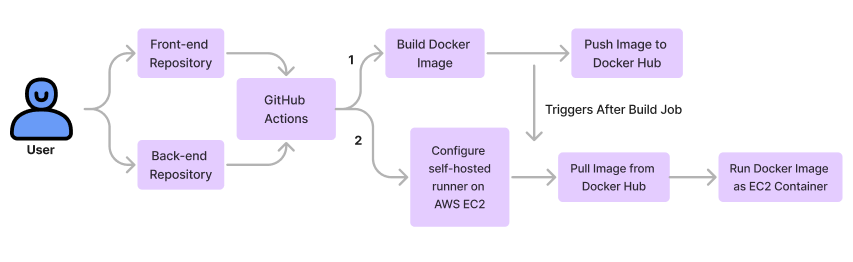
\includegraphics[width=1\linewidth]{cloud-deployment.png}
    \caption{Schematische Visualisierung des Deploymentprozesses}
    \label{fig:enter-label}
\end{figure}

\subsection{Cloud Deployment}
Das Projekt nutzt AWS für die Bereitstellung im Cloud-Umfeld. Folgende AWS-Dienste werden verwendet:

\begin{itemize}
  \item \textbf{AWS Route 53:} Konfiguriert, um die Domain `munchmunch.tech` zu verwalten.
  \item \textbf{EC2 Instanzen:} Hosting der Anwendung auf Amazon Linux 2 EC2-Instanzen.
  \item \textbf{IAM Identity Center:} Verwaltet die Berechtigungen und Zugänge für die AWS-Ressourcen, sowie Zugänge zur AWS Konsole für alle Teammitglieder unter einer Root-Domäne.
\end{itemize}

Ein `.env production file` wird verwendet, um die Umgebungsvariablen im Produktionsmodus sicher zu handhaben.

\section{Entwicklungswerkzeuge}
\subsection{Express.js}
Express.js ist ein node-basiertes HTTP-Framework. Es wird für die Kommunikation zwischen dem Frontend und der Datenbank verwendet. Dazu nutzt es eine Verbindung zur Datenbank über die MongoDB Bibliothek. Mithilfe einer RESTful API werden die Daten über verschiedene Routen mit GET-Methoden geliefert. Um neue Daten zu der Datenbank hinzufügen zu können, oder bestehende Daten zu aktualisieren, wird die HTTP POST-Methode verwendet.

\subsection{Nodemon}
Nodemon überwacht die Dateien im Server-Verzeichnis auf Änderungen. Falls die Änderungen gespeichert werden, wird der Backend-Server neu gestartet. Der Hot-Reload-Service von Nodemon unterstützt den Entwicklungsprozess und das Debugging durch detaillierte Fehlerausgaben bei Neukompillierung. 

\subsection{Bcrypt}
Bcrypt.js ist eine Krypto-Bibliothek, welche unter Anderem die bcrypt Hashfunktion implementiert. Es wird im Authentifizierungsmodul verwendet, um Passwörter der Benutzer in einem geheimen Text umwandeln zu können, um einen Standard von Sicherheit zu gewährleisten.

\subsection{Infrastruktur und TypeScript}
TypeScript wird im gesamten Projekt verwendet, um die Typsicherheit zu verbessern und die Entwicklung zu vereinfachen. Es hilft besonders bei der Definition von Datenmodellen und der sicheren Handhabung von Datentransaktionen zwischen Frontend und Backend, via der HTTP-Aufrufe innerhalb der Frontend Service-Klassen auf die RESTful API des Backends, welche innerhalb der Backend Routing-Middlewares implementiert sind.

\subsection{Tailwind.css und Vite}
Für das Styling der Benutzeroberfläche wird Tailwind.css\cite{TailwindCSS} verwendet, welches effizientes und responsives Design durch Utility-first CSS-Klassen ermöglicht. Vite wird als Build-Tool und Entwicklungsserver eingesetzt, um schnelle Wiederaufbauprozesse und eine optimierte Entwicklungsperformance zu gewährleisten.

\subsection{Axios}
Axios wird als HTTP-Client genutzt, um Kommunikation zwischen dem Frontend und dem Backend zu ermöglichen. Es unterstützt das Projekt durch die einfache Handhabung von Netzwerkanfragen und das Verarbeiten von JSON-Daten.

\section {Fazit und Ausblick} 
Mit der erfolgreichen Implementierung des MVPs von MunchMunch wurde eine solide Grundlage geschaffen, um die kulinarische Bildung zu fördern und das Kocherlebnis zu optimieren. Die Anwendung ermöglicht es den Nutzern, mühelos neue Gerichte zu entdecken, Rezepte zu speichern und personalisierte Kochanleitungen zu nutzen. Dank der Verwendung des MERN-Stacks konnten wir eine robuste und skalierbare Plattform entwickeln, die sowohl auf Heimcomputern als auch auf mobilen Geräten nutzbar ist.

Für die Zukunft sind folgende Erweiterungen geplant, um das Nutzererlebnis weiter zu verbessern:
\begin{enumerate}
\item Einkaufsliste: Als Nutzer möchte ich die Zutaten aus einem Rezept in einer Einkaufsliste speichern können, damit ich beim Einkaufen direkt die benötigten Zutaten sehen kann.
\begin{enumerate}
\item  Ein Button in einem Rezept zum Speichern der Zutaten wird angezeigt.
\item  Die Zutaten werden in einer Einkaufsliste, die ein weiterer Menüpunkt ist, gespeichert.
\item  Die Einkaufsliste mit den gespeicherten Zutaten kann jederzeit angesehen werden.
\end{enumerate}

\item Alternativer Entdeckermodus: Als Nutzer möchte ich einen spielerischen Modus haben, in dem mir jeweils nur ein einzelnes Rezept vorgeschlagen wird.
\begin{enumerate}
\item Beim Wischen nach rechts wird ein Match angezeigt und das Gericht in den Favoriten gespeichert.
\item Beim Wischen nach links wird das Nichtgefallen eines Rezepts ausgedrückt und das Gericht wird in Zukunft weniger angezeigt.
\item In den alternativen Modus kann bei Bedarf auf der Übersicht gewechselt werden.
\end{enumerate}

\item Anzeige der bisher gekochten Rezepte: Als Nutzer möchte ich sehen, welche Rezepte ich bereits gekocht habe, damit ich auch mal Neues ausprobieren kann, aber trotzdem in der Lage bin, diese nochmals zu kochen.
\begin{enumerate}
\item Rezepte können mit "Gekocht" gekennzeichnet werden.
\item Gekochte Rezepte werden nicht mehr bei den normalen Vorschlägen angezeigt.
\item Es gibt eine eigene Kategorie, in der die bereits gekochten Rezepte angezeigt werden.
\end{enumerate}


\item KI-Chatbot: Als Nutzer möchte ich einen integrierten KI-Chatbot haben, dem ich verschiedene Dinge schreiben kann, damit er mir dafür ein passendes Rezept heraussucht.
\begin{enumerate}
\item Der KI-Chatbot wird als weiterer Menüpunkt angezeigt.
\item Der KI-Chatbot hat ein Eingabefeld, um ihm Nachrichten zu schreiben.
\item Der KI-Chatbot zeigt das passende Rezept dazu an.
\item Das Rezept kann in die Favoritenliste gespeichert werden.
\end{enumerate}
\end{enumerate}

%%% Previous TechReps
\nocite{ModA-TR-2023SS-WAE-TeamWeiss-Neunerln}
\nocite{ModA-TR-2023SS-BDCC-TeamRot-CompVisPipeline}
\nocite{ModA-TR-2023SS-BDCC-TeamBlau-NauticalNonsense}
\nocite{ModA-TR-2023SS-BCN-TeamGruen-TorpedoTactics}
\nocite{ModA-TR-2023SS-BCN-TeamCyan-Stockbird}
\nocite{ModA-TR-2023SS-BCN-TeamBlau-FancyChess}
\nocite{ModA-TR-2023WS-SWT-TeamRot-SGDb}
\nocite{ModA-TR-2023WS-SWT-TeamGruen-OPCUANetzwerk}
\nocite{ModA-TR-2022SS-WAE-TeamWeiss-WoIstMeinGeld}
\nocite{ModA-TR-2022SS-BDCC-TeamWeiss-TwitterDash}
\nocite{ModA-TR-2022SS-BDCC-TeamRot-Reddiment}
\nocite{ModA-TR-2022SS-BDCC-TeamGruen-ExplosionGuy}
\nocite{ModA-TR-2022SS-BDCC-TeamCyan-OTHWiki}
\nocite{ModA-TR-2022WS-SWT-TeamGruen-Graphvio}
\nocite{ModA-TR-2021SS-WAE-TeamWeiss-CovidDashboard}
\nocite{ModA-TR-2021SS-WAE-TeamRot-FireForceDefense}
\nocite{ModA-TR-2021SS-WAE-TeamGruen-MedPlanner}

%%% Misc

\nocite{Amazon}
\nocite{Netflix}
\nocite{EATCLUB}
\nocite{Node.js}
\nocite{MongoDB}
\nocite{Express}
\nocite{Vite}
\nocite{TypeScript}
\nocite{React.js}
\nocite{Docker}
\nocite{TailwindCSS}

% Print bibliography excluding self references
\printbibliography[notcategory=selfref]

\end{document}